\section{Referencia de la Clase Informe\-Clientes}
\label{classInformeClientes}\index{InformeClientes@{InformeClientes}}
Genera un informe de todos los cliente.  


{\tt \#include $<$informereferencia.h$>$}

Diagrama de colaboraci\'{o}n para Informe\-Clientes:\begin{figure}[H]
\begin{center}
\leavevmode
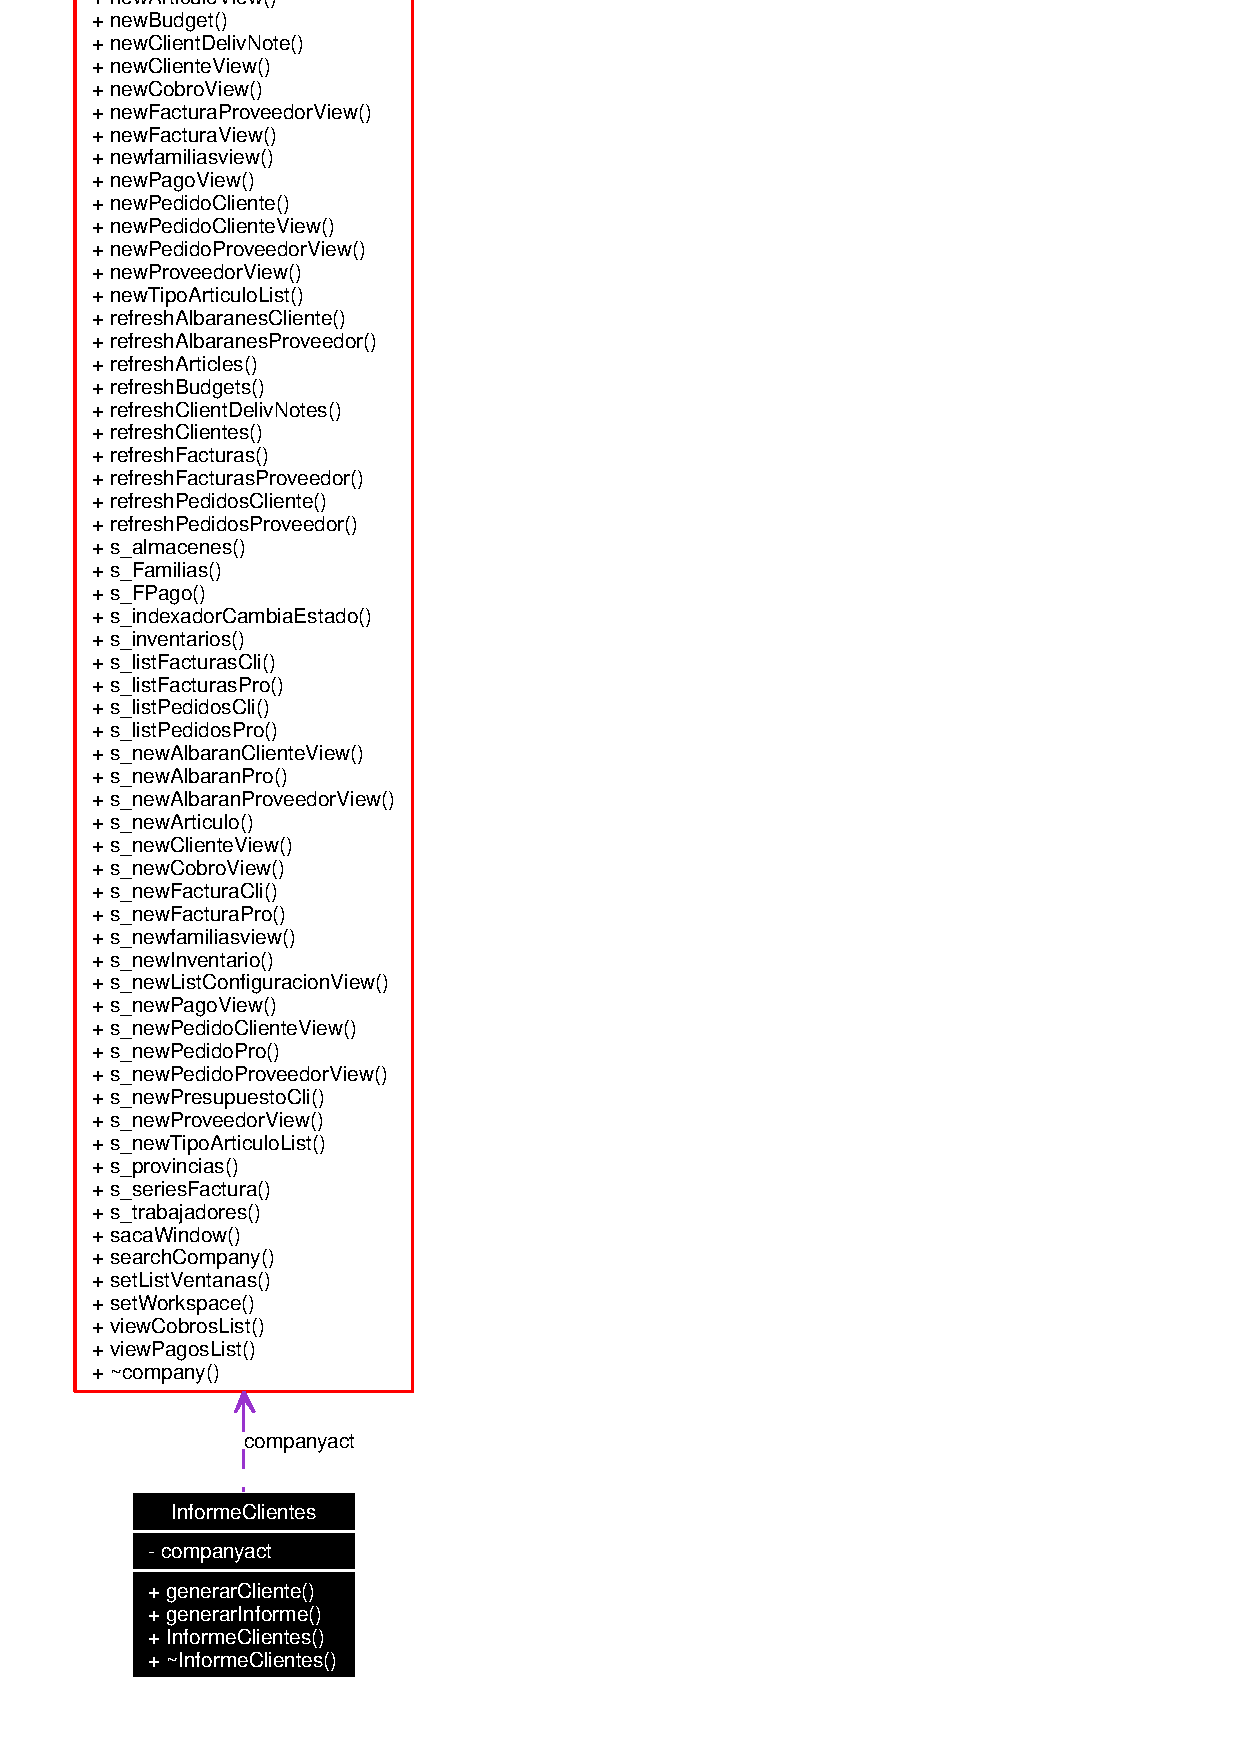
\includegraphics[width=99pt]{classInformeClientes__coll__graph}
\end{center}
\end{figure}
\subsection*{M\'{e}todos p\'{u}blicos}
\begin{CompactItemize}
\item 
QString {\bf generar\-Cliente} (QString)
\item 
void {\bf generar\-Informe} ()
\item 
{\bf Informe\-Clientes} ({\bf company} $\ast$)
\end{CompactItemize}


\subsection{Descripci\'{o}n detallada}
Genera un informe de todos los cliente. 



\subsection{Documentaci\'{o}n del constructor y destructor}
\index{InformeClientes@{Informe\-Clientes}!InformeClientes@{InformeClientes}}
\index{InformeClientes@{InformeClientes}!InformeClientes@{Informe\-Clientes}}
\subsubsection{\setlength{\rightskip}{0pt plus 5cm}Informe\-Clientes::Informe\-Clientes ({\bf company} $\ast$ {\em comp})}\label{classInformeClientes_a2}


================================================================ =================== INFORME CLIENTES ============================ ================================================================ 

\subsection{Documentaci\'{o}n de las funciones miembro}
\index{InformeClientes@{Informe\-Clientes}!generarCliente@{generarCliente}}
\index{generarCliente@{generarCliente}!InformeClientes@{Informe\-Clientes}}
\subsubsection{\setlength{\rightskip}{0pt plus 5cm}QString Informe\-Clientes::generar\-Cliente (QString {\em idcliente})}\label{classInformeClientes_a0}


Sacamos todas las referencias de este cliente y las guardamos en el string referencias

Generacion del informe de ventas.

Generacion del informe de compras.

Generacion del informe de totales de ventas.

Calculo de las cantidades totales en moneda.

Total presupuestado.

Total pedido.

Total trabajado.

Total facturado.

Total cobrado.

Generacion del informe de totales de compras.

Calculo de las cantidades totales en moneda.

Total pedido.

Total trabajado.

Total facturado.

Total cobrado. \index{InformeClientes@{Informe\-Clientes}!generarInforme@{generarInforme}}
\index{generarInforme@{generarInforme}!InformeClientes@{Informe\-Clientes}}
\subsubsection{\setlength{\rightskip}{0pt plus 5cm}void Informe\-Clientes::generar\-Informe ()}\label{classInformeClientes_a1}


Copiamos el archivo.

Copiamos el logo.

Sacamos los datos del cliente. 

La documentaci\'{o}n para esta clase fu\'{e} generada a partir de los siguientes archivos:\begin{CompactItemize}
\item 
informereferencia.h\item 
informereferencia.cpp\end{CompactItemize}
